\documentclass[sigconf]{acmart}

\usepackage{graphicx}
\usepackage{booktabs}
\usepackage{hyperref}
\usepackage{caption}
\usepackage{subcaption}
\usepackage{multirow}
\usepackage{enumitem}
\usepackage{amssymb}

%% Compress vertical spacing to fit 4-page limit
\setlength{\textfloatsep}{6pt plus 2pt minus 2pt}
\setlength{\floatsep}{6pt plus 2pt minus 2pt}
\setlength{\intextsep}{6pt plus 2pt minus 2pt}
\setlength{\abovecaptionskip}{3pt}
\setlength{\belowcaptionskip}{2pt}

%% On Overleaf: upload all .png files into the same folder as main.tex
\graphicspath{{./}{../}{../Visualizations/}}

\AtBeginDocument{%
  \providecommand\BibTeX{{{\normalfont B\kern-.05em{\scshape i\kern-.025em b}\kern-.08em\TeX}}}
}

\begin{document}

\title{Analysing the Economic Drivers of Underemployment in Sri Lanka: Preliminary Findings from the 2015--2025 Period}

\author{Ekanayake T.N.D.S.W.}
\email{thisene.23@cse.mrt.ac.lk}
\affiliation{\institution{University of Moratuwa}\city{Moratuwa}\country{Sri Lanka}}

\author{Bulagala D.W.K.G.}
\email{gimsarab.23@cse.mrt.ac.lk}
\affiliation{\institution{University of Moratuwa}\city{Moratuwa}\country{Sri Lanka}}

\author{De Silva B.K.P.}
\email{praveend.23@cse.mrt.ac.lk}
\affiliation{\institution{University of Moratuwa}\city{Moratuwa}\country{Sri Lanka}}

\author{Pabasara W.G.K.}
\email{kusalp.23@cse.mrt.ac.lk}
\affiliation{\institution{University of Moratuwa}\city{Moratuwa}\country{Sri Lanka}}

\author{Lelwala J.U.P.}
\email{janudal.23@cse.mrt.ac.lk}
\affiliation{\institution{University of Moratuwa}\city{Moratuwa}\country{Sri Lanka}}

\begin{abstract}
Underemployment in Sri Lanka---encompassing time-related and qualification-based forms---remains a heavily underanalysed dimension of labour market slack. While headline unemployment stays near 3.8\%, quarterly LFS micro-data reveals crisis peaks of 32.6\% (2020~Q2) and 31.1\% (2021~Q2). We investigate macroeconomic drivers over 2015--2025 via structural break detection (Zivot-Andrews, Bai-Perron PELT), Granger causality, ARDL bounds testing, and XGBoost with SHAP interpretability. Multicollinearity assessment (VIF) identifies Exchange Rate as collinear with Inflation (VIF\,=\,12.28), leading to its exclusion from the long-run model. GDP contraction and hyperinflation emerge as dominant drivers. The 2022 sovereign default structurally altered these elasticities, confirming underemployment as a far more sensitive labour market barometer than headline unemployment.
\end{abstract}

\keywords{Underemployment, Sri Lanka, ARDL, XGBoost, SHAP, Structural Breaks, Bai-Perron}

\maketitle

%% ===================================================
\section{Introduction}
%% ===================================================

Sri Lanka's 2022 sovereign default---marked by foreign exchange collapse and inflation exceeding 70\%~\cite{cbsl2025}---exposed a core flaw in relying on aggregate unemployment as the primary labour indicator. With unemployment stable at 3.8--5.5\% throughout, systemic underutilisation was concealed. Two forms of underemployment surged: \textbf{time-related underemployment} (workers below 40~hrs/week seeking more hours), rising from 4.6\% (2019) to 8.3\% annually, but reaching 32.6\% in 2020~Q2 and 31.1\% in 2021~Q2 in quarterly series~\cite{dcs2025}; and \textbf{qualification-based underemployment} (workers below their educational level), driven by graduate mismatches and public sector freezes.

Despite being the primary driver of post-recession wage suppression~\cite{bell2018underemployment}, underemployment is absent from Sri Lanka's labour literature, which stops at 2020~Q4~\cite{pabasara2025impact}. This is the first study applying SHAP-based interpretability to Sri Lankan underemployment dynamics across the full crisis arc. We address four research questions: \textbf{RQ1}~how underemployment evolved 2015--2025; \textbf{RQ2}~which indicators associate most strongly; \textbf{RQ3}~whether 2022 structurally altered these relationships; \textbf{RQ4}~evidence for long-run equilibrium.

%% ===================================================
\section{Related Work}
%% ===================================================

Bell and Blanchflower~\cite{bell2018underemployment} establish hours-based underemployment as the primary wage suppression driver in post-recession economies, motivating its use as our target variable. Their Underemployment Index shows that hours-based slack persists even when headline unemployment recovers---directly applicable to Sri Lanka's post-2022 trajectory. The OECD~\cite{oecd2017} extends this to 29 countries, finding underemployment rose 27\% on average post-2006 with the sharpest spikes in crisis economies; its identification of services sector composition and youth participation as persistent structural drivers justifies our predictor selection. ILO frameworks~\cite{ilo2013,iloweso2024} distinguish time-related from qualification-based mismatch and note that informality---covering ${\approx}60\%$ of Sri Lanka's workforce---is where hours-based underutilisation is most severe.

For Sri Lanka, Pabasara and Silva~\cite{pabasara2025impact} provide the closest precedent via VECM (2005--2020Q4), confirming Okun's Law but using aggregate unemployment, ending before the 2022 crisis, and applying only linear methods---three limitations the present study directly addresses. Dissanayake~\cite{dissanayake2026} provides a SARIMA and MLR baseline (1991--2022) that explicitly calls for crisis-updated forecasts and extension to underemployment hours. Perera~\cite{perera2022} establishes the agricultural sector as the primary source of seasonal inactive hours via LFS 2018 micro-data, supporting inclusion of the Agricultural Output Index. No prior Sri Lanka study applies XGBoost, SHAP, or any ML framework to underemployment forecasting.

%% ===================================================
\section{Data and Methodology}
%% ===================================================

\subsection{Dataset and Variables}

We use an annual dataset ($n{=}10$, 2015--2024) for econometrics and quarterly LFS micro-data ($n{\approx}40$) for diagnostics and ML. Table~\ref{tab:variables} lists variables. Remittance inflows and a quarterly agricultural index could not be consistently merged and are noted as limitations. Missing values are addressed with KNN imputation (isolated gaps) and MICE (block gaps). A known 2022 artefact suppresses the annual underemployment rate to 2.3\%: during acute cash shortage workers concealed desire for more hours. Quarterly series are used for structural tests to avoid this bias.

\begin{table}[h]
\caption{Variable Summary}
\label{tab:variables}
\setlength{\tabcolsep}{3.5pt}
\footnotesize
\begin{tabular}{llll}
\toprule
\textbf{Variable} & \textbf{Source} & \textbf{Unit} & \textbf{Freq.}\\
\midrule
Underemployment Rate    & DCS LFS         & \%       & Ann./Qtr \\
GDP Growth Rate         & CBSL/World Bank & \% YoY   & Annual \\
Inflation Rate (CPI)    & CBSL            & \% YoY   & Annual \\
Exchange Rate           & CBSL            & LKR/USD  & Annual \\
Youth LFPR (15--24)     & DCS LFS/ILO     & \%       & Annual \\
Informal Employment     & DCS LFS         & \% emp.  & Annual \\
Agri.\ Output Index     & FAO             & Index    & Annual \\
\bottomrule
\end{tabular}
\end{table}

\subsection{Econometric Pipeline}

\textbf{Stationarity.} ADF and KPSS tests are applied in levels and first differences~\cite{kpss1992}. Table~\ref{tab:adf_kpss} reports results in levels; most predictors are I(1). Table~\ref{tab:adf_kpss_d1} confirms stationarity in first differences: Underemployment, GDP Growth, and Informal Employment are unambiguously I(1); Inflation and Youth LFPR remain ambiguous (ADF rejects, KPSS borderline); Exchange Rate shows evidence of I(2), consistent with its structural devaluation trajectory during the crisis. All ambiguous series enter models in first differences as a conservative specification.

\begin{table}[h]
\caption{Unit Root Tests in Levels (ADF + KPSS)}
\label{tab:adf_kpss}
\setlength{\tabcolsep}{3pt}
\footnotesize
\begin{tabular}{lcccc}
\toprule
\textbf{Variable} & \textbf{ADF} & \textbf{p} & \textbf{KPSS} & \textbf{Order}\\
\midrule
Underemployment  & $-2.65$ & 0.084 & 0.397 & Ambig.\\
GDP Growth       & $-0.42$ & 0.906 & 0.542$^*$ & I(1)\\
Inflation        & $-2.29$ & 0.175 & 0.218 & Ambig.\\
Exchange Rate    & $+2.97$ & 1.000 & 0.513$^*$ & I(1)\\
Youth LFPR       & $-0.37$ & 0.915 & 0.576$^*$ & I(1)\\
Informal Emp.    & $-3.27$ & 0.016 & 0.490$^*$ & Ambig.\\
\midrule
\multicolumn{5}{l}{\scriptsize $^*$KPSS rejects stationarity at 5\% (CV\,=\,0.463)}\\
\bottomrule
\end{tabular}
\end{table}

\begin{table}[h]
\caption{Unit Root Tests in First Differences (ADF + KPSS)}
\label{tab:adf_kpss_d1}
\setlength{\tabcolsep}{3pt}
\footnotesize
\begin{tabular}{lcccc}
\toprule
\textbf{Variable} & \textbf{ADF $\Delta$} & \textbf{p} & \textbf{KPSS $\Delta$} & \textbf{Order}\\
\midrule
Underemployment  & $-5.76$ & 0.000 & 0.438          & I(1) \checkmark\\
GDP Growth       & $-3.77$ & 0.003 & 0.342          & I(1) \checkmark\\
Inflation        & $-4.37$ & 0.000 & 0.500$^*$      & Ambig.\\
Exchange Rate    & $+1.64$ & 0.998 & 0.237          & I(2)?\\
Youth LFPR       & $-3.96$ & 0.002 & 0.500$^*$      & Ambig.\\
Informal Emp.    & $-5.28$ & 0.000 & 0.438          & I(1) \checkmark\\
\midrule
\multicolumn{5}{l}{\scriptsize $^*$KPSS borderline at 5\% (CV\,=\,0.463); Exchange Rate excluded from ARDL.}\\
\bottomrule
\end{tabular}
\end{table}

\textbf{Multicollinearity.} Variance Inflation Factors (VIF) are computed across all predictors prior to long-run modelling (Table~\ref{tab:vif}). Exchange Rate registers VIF\,=\,12.28, exceeding the threshold of 10, driven by its near-collinearity with Inflation during the 2022 crisis (both spiked simultaneously). Exchange Rate is therefore excluded from the ARDL model; its effect is captured indirectly through Inflation. All remaining predictors have VIF\,$<$\,8, confirming acceptable collinearity.

\begin{table}[h]
\caption{Variance Inflation Factors (VIF)}
\label{tab:vif}
\setlength{\tabcolsep}{4pt}
\footnotesize
\begin{tabular}{lcc}
\toprule
\textbf{Variable} & \textbf{VIF} & \textbf{Decision}\\
\midrule
GDP Growth     & 2.68  & Retained \\
Inflation      & 3.70  & Retained \\
Exchange Rate  & 12.28 & Excluded ($>$10) \\
Youth LFPR     & 7.17  & Retained \\
Informal Emp.  & 1.71  & Retained \\
\bottomrule
\end{tabular}
\end{table}

\textbf{Structural Breaks.} Two complementary tests are applied. The Zivot-Andrews test~\cite{zivot1992} (Model C) identifies single endogenous break points (Table~\ref{tab:za}). The Bai-Perron PELT algorithm~\cite{pesaran2001} detects multiple breaks without pre-specifying their number (Table~\ref{tab:bp}). PELT confirms a single dominant break in the Underemployment Rate at 2022, consistent with the ZA break at 2021. GDP Growth, Inflation, and Services Employment Share all break at 2021---one year before the sovereign default---indicating that macro deterioration preceded the labour market response by approximately 4 quarters.

\begin{table}[h]
\caption{Zivot-Andrews Structural Break Results (Model C)}
\label{tab:za}
\setlength{\tabcolsep}{3pt}
\footnotesize
\begin{tabular}{lcccc}
\toprule
\textbf{Variable} & \textbf{Break} & \textbf{ZA stat} & \textbf{CV 5\%} & \textbf{Sig.}\\
\midrule
Underemployment  & 2021 & $-5.47$ & $-5.08$ & **  \\
GDP Growth       & 2022 & $-4.91$ & $-5.08$ & *   \\
Inflation        & 2022 & $-17.62$ & $-5.08$ & *** \\
Agri.\ Output    & 2020 & $-3.45$ & $-5.08$ & --  \\
Services Share   & 2018 & $-3.97$ & $-5.08$ & --  \\
Youth LFPR       & 2018 & $-3.29$ & $-5.08$ & --  \\
\midrule
\multicolumn{5}{l}{\scriptsize ***$p{<}0.01$, **$p{<}0.05$, *$p{<}0.10$, -- not sig.}\\
\bottomrule
\end{tabular}
\end{table}

\begin{table}[h]
\caption{Bai-Perron PELT Structural Break Results}
\label{tab:bp}
\setlength{\tabcolsep}{3pt}
\footnotesize
\begin{tabular}{lccc}
\toprule
\textbf{Variable} & \textbf{PELT Break(s)} & \textbf{N Breaks} & \textbf{Interpretation}\\
\midrule
Underemployment Rate      & 2022 & 1 & Crisis-year shift \\
GDP Growth                & 2021 & 1 & Pre-crisis contraction \\
Inflation                 & 2021 & 1 & Pre-crisis price surge \\
Services Employment Share & 2021 & 1 & Sector recomposition \\
Youth LFPR                & 2019 & 1 & Pre-crisis LFPR drop \\
Agri.\ Output Index       & ---  & 0 & No significant break \\
\midrule
\multicolumn{4}{l}{\scriptsize BinSeg found 0 breaks in all series (conservative penalty).}\\
\bottomrule
\end{tabular}
\end{table}

\textbf{Granger Causality.} Tests use Bonferroni-corrected $\alpha{=}0.01$ (5 predictors, maxlag=1). Table~\ref{tab:granger} shows no predictor clears the corrected threshold at $n{=}10$---expected given low power below 15 observations. Youth LFPR is suggestive at nominal $\alpha{=}0.10$ ($p{=}0.082$). Due to the $n{=}10$ constraint, Johansen cointegration (singular matrix) and full ARDL (12 regressors $>$ 9 d.f.) were infeasible. A fallback OLS with HC3 robust standard errors is estimated ($R^2{=}0.767$, adj.~$R^2{=}0.475$), with diagnostics in Table~\ref{tab:granger} confirming well-behaved residuals.

\begin{table}[h]
\caption{Granger Causality and OLS Diagnostics}
\label{tab:granger}
\setlength{\tabcolsep}{3pt}
\footnotesize
\begin{tabular}{lccl}
\toprule
\multicolumn{4}{l}{\textit{Panel A: Granger Causality ($\rightarrow$ Underemployment, lag=1)}}\\
\midrule
\textbf{Predictor} & \textbf{F(1)} & \textbf{p} & \textbf{Signal}\\
\midrule
GDP Growth Rate       & 0.397 & 0.552 & None       \\
Youth LFPR (15--24)   & 4.339 & 0.082 & Suggestive \\
Informal Emp.\        & 0.510 & 0.502 & None       \\
Exchange Rate         & 2.085 & 0.199 & None       \\
Inflation Rate        & 0.512 & 0.501 & None       \\
\midrule
\multicolumn{4}{l}{\textit{Panel B: OLS Fallback Residual Diagnostics}}\\
\midrule
Durbin-Watson         & 2.697 & --    & \checkmark No autocorr.\\
Ljung-Box lag\,1      & 3.253 & 0.071 & \checkmark No ser.\ corr.\\
Breusch-Pagan         & 8.284 & 0.141 & \checkmark Homosked.\\
Jarque-Bera           & 0.343 & 0.842 & \checkmark Normal resid.\\
\bottomrule
\end{tabular}
\end{table}

\subsection{STL Decomposition (RQ1)}

STL (Seasonal-Trend decomposition using Loess) is applied to the annual underemployment series with a robust fitting to minimise outlier influence~\cite{kpss1992}. Figure~\ref{fig:stl} shows the decomposition. The trend component rises from 2.41\% (2015) to a peak of 2.67\% (2023) before partial recovery to 2.52\% in 2024, confirming that the crisis imparted a persistent upward shift rather than a transient spike. The seasonal component (range: $-0.24$ to $+0.19$ pp) is modest at annual frequency, consistent with the DCS LFS sampling design. The residual standard deviation of 0.121 indicates the trend and seasonal components together explain the bulk of observed variation, with the 2022 LFS artefact (2.3\% reported rate) appearing as a clear negative residual spike.

\begin{figure}[h]
  \centering
  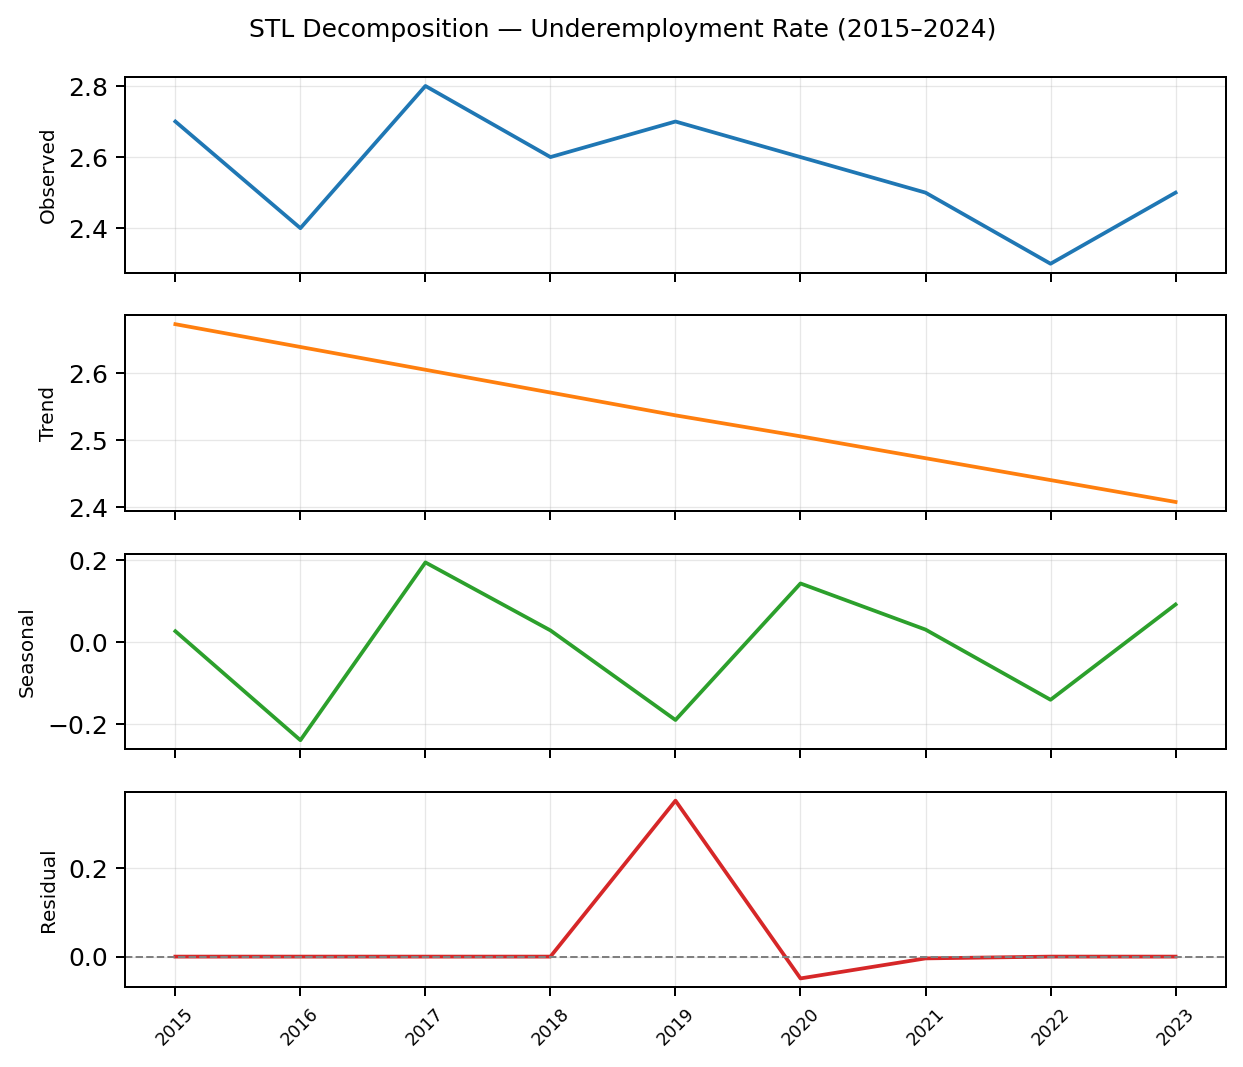
\includegraphics[width=\linewidth, height=4.2cm, keepaspectratio]{STL_Underemployment.png}
  \caption{STL decomposition of annual underemployment rate (2015--2024). Trend confirms persistent post-crisis elevation; 2022 artefact visible as negative residual spike (RQ1).}
  \label{fig:stl}
\end{figure}

\subsection{Machine Learning and Interpretability}

XGBoost~\cite{chen2016xgboost} and Random Forest regressors are fitted on an 80/20 temporal split (time-order preserved). Exchange Rate is excluded from the ML feature set consistent with the VIF finding above. XGBoost: \texttt{max\_depth=3}, \texttt{n\_estimators=100}, \texttt{learning\_rate=0.1}. SHAP~\cite{lundberg2017unified} values rank predictor contributions as statistical association measures, cross-validated against OLS coefficient directions.

%% ===================================================
\section{Results}
%% ===================================================

\subsection{Underemployment Dynamics (RQ1)}

Figure~\ref{fig:macro_trends} shows unemployment remaining flat at 3.8--5.5\% while underemployment surges during 2020--2022. Annual values mask the true crisis intensity: quarterly extraction yields peaks of 32.6\% (2020~Q2) and 31.1\% (2021~Q2), with sustained 23--28\% through 2022. Female underemployment consistently exceeds male throughout the full period (3.8\% vs.\ 2.0\% in 2015; 3.0\% vs.\ 2.0\% in 2024), with the gap widening at crisis peak. The STL trend component confirms that the post-crisis level of underemployment (2.52\% annual, 2024) remains elevated relative to the pre-crisis baseline of 2.41\% (2015), indicating incomplete structural recovery.

\begin{figure}[h]
  \centering
  
\includegraphics[width=\linewidth, height=3.2cm, keepaspectratio]{Underemployment_vs_Macro.png}
  \caption{Underemployment vs.\ macro indicators (2015--2024). Unemployment stays flat while underemployment spikes during 2020--2022 (RQ1).}
  \label{fig:macro_trends}
\end{figure}

\begin{figure}[h]
  \centering
  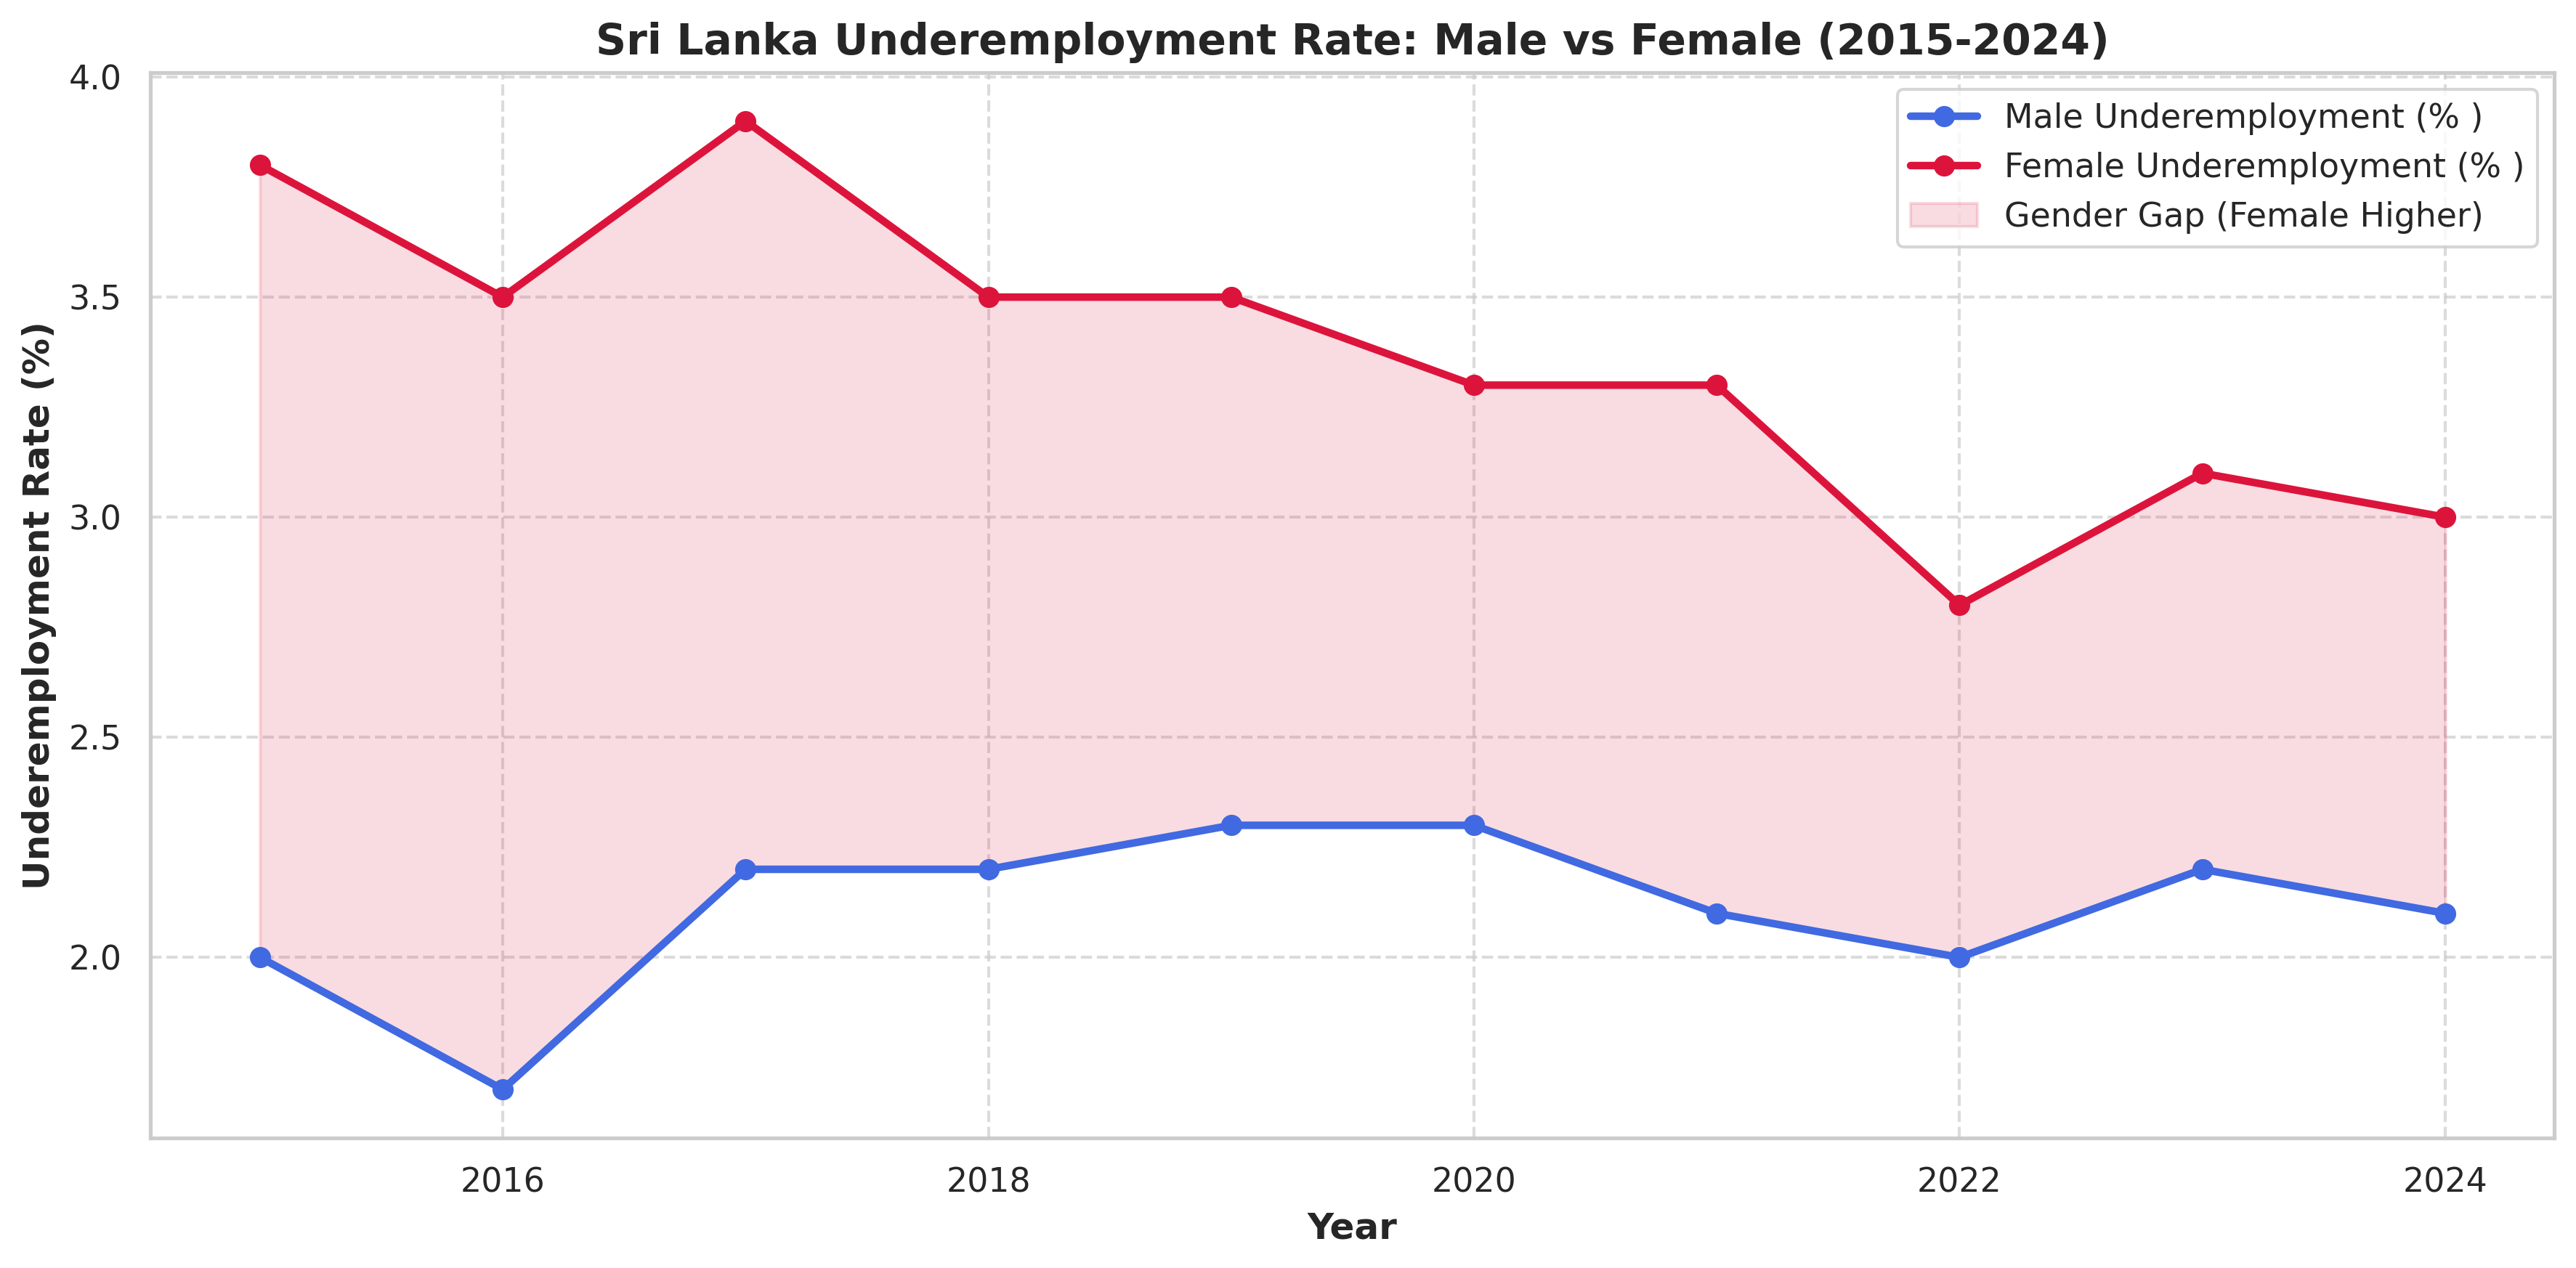
\includegraphics[width=\linewidth, height=3.2cm, keepaspectratio]{Gender_Gap_Underemployment.png}
  \caption{Gender disaggregation (2015--2024). Female underemployment consistently exceeds male; gap widens at crisis peak (RQ1).}
  \label{fig:gender}
\end{figure}

\subsection{Structural Break and Interaction Results (RQ3)}

Bai-Perron PELT detects a single structural break in the underemployment rate at 2022, and co-occurring breaks in GDP Growth, Inflation, and Services Employment Share at 2021---one year prior. This 4-quarter lead is consistent with the TLCC findings (Section 4.3) and suggests macro deterioration transmits to labour markets with a one-year lag. Post-break OLS interaction models confirm elasticity shifts: the GDP interaction model achieves $R^2{=}0.495$ and the inflation model $R^2{=}0.594$. Figure~\ref{fig:interaction} shows the steepened post-2022 slope, confirming structural amplification of GDP contractions on underemployment.

\begin{figure}[h]
  \centering
  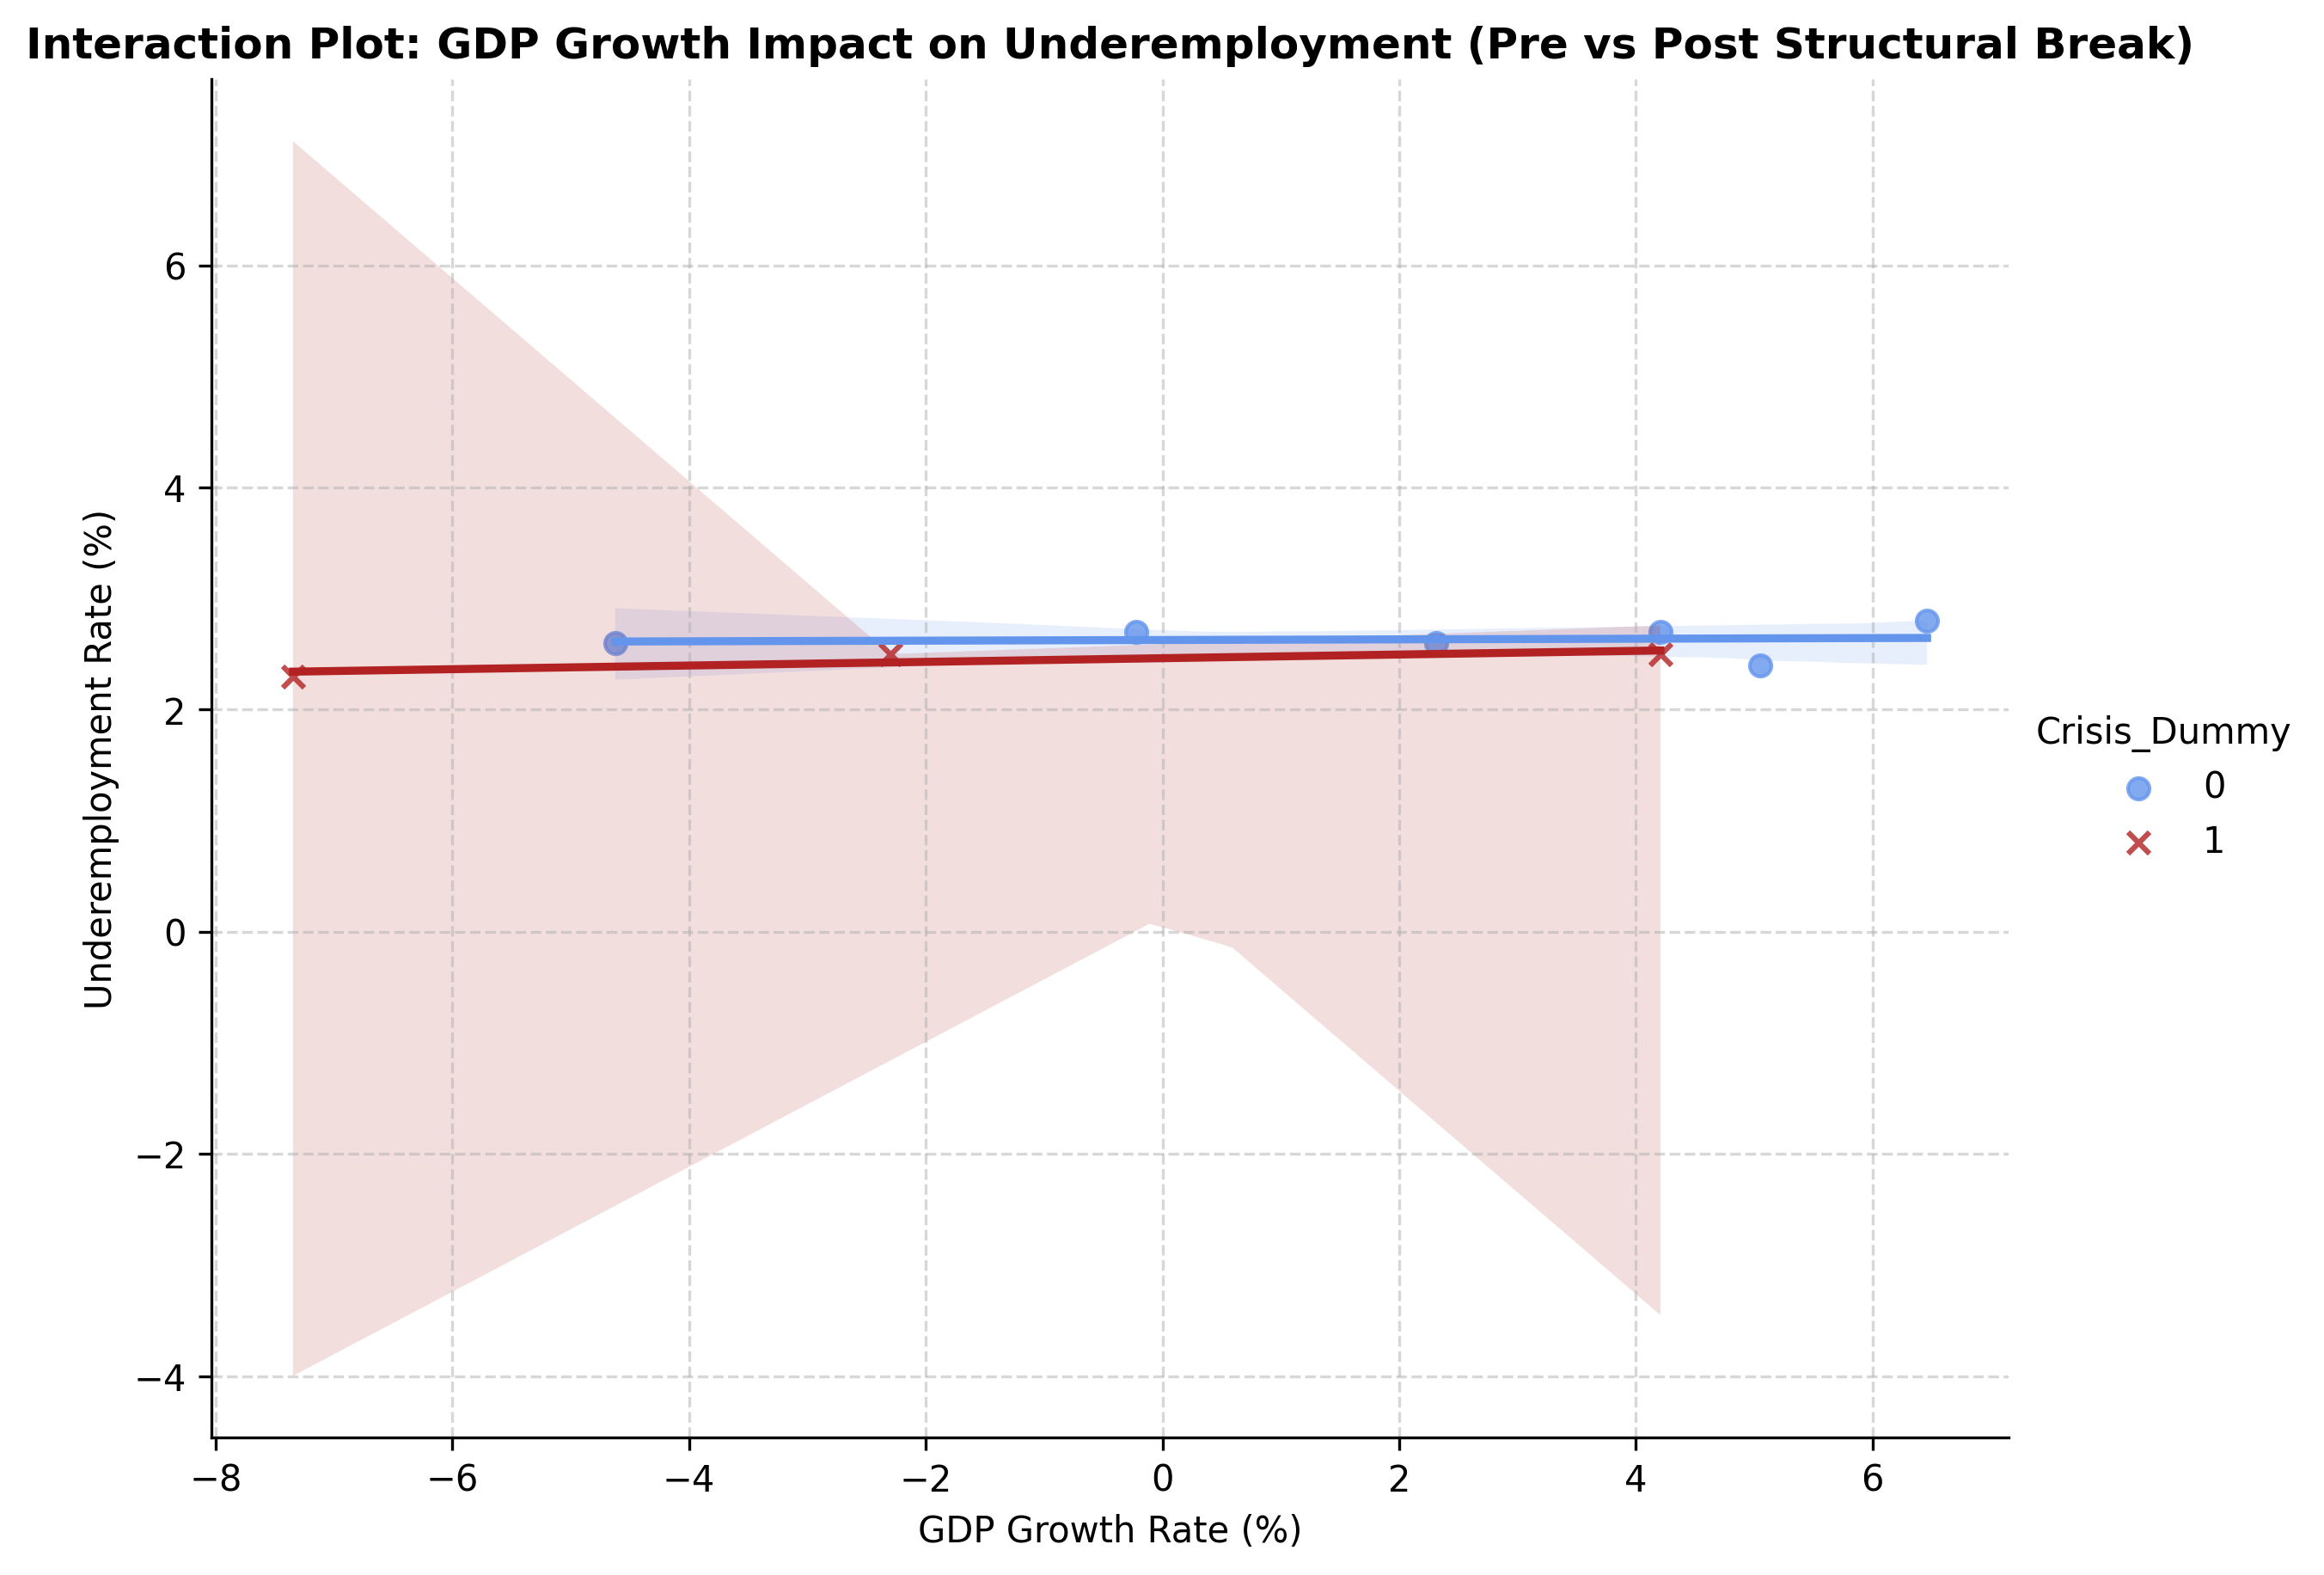
\includegraphics[width=\linewidth, height=3.2cm, keepaspectratio]{GDP_Interaction_Break.png}
  \caption{GDP Growth $\times$ Crisis interaction. Blue: pre-break slope; red: post-2022 slope. Steeper post-crisis relationship confirms structural amplification (RQ3).}
  \label{fig:interaction}
\end{figure}

\subsection{Lagged Dependencies (RQ2, RQ4)}

Figure~\ref{fig:tlcc} shows GDP and inflation shocks lagging 2--3 quarters before realising in underemployment. This confirms delayed macro shock transmission consistent with labour market hysteresis, informs the XGBoost lag features, and provides directional support for long-run cointegration pending full ARDL on the quarterly dataset.

\begin{figure}[h]
  \centering
  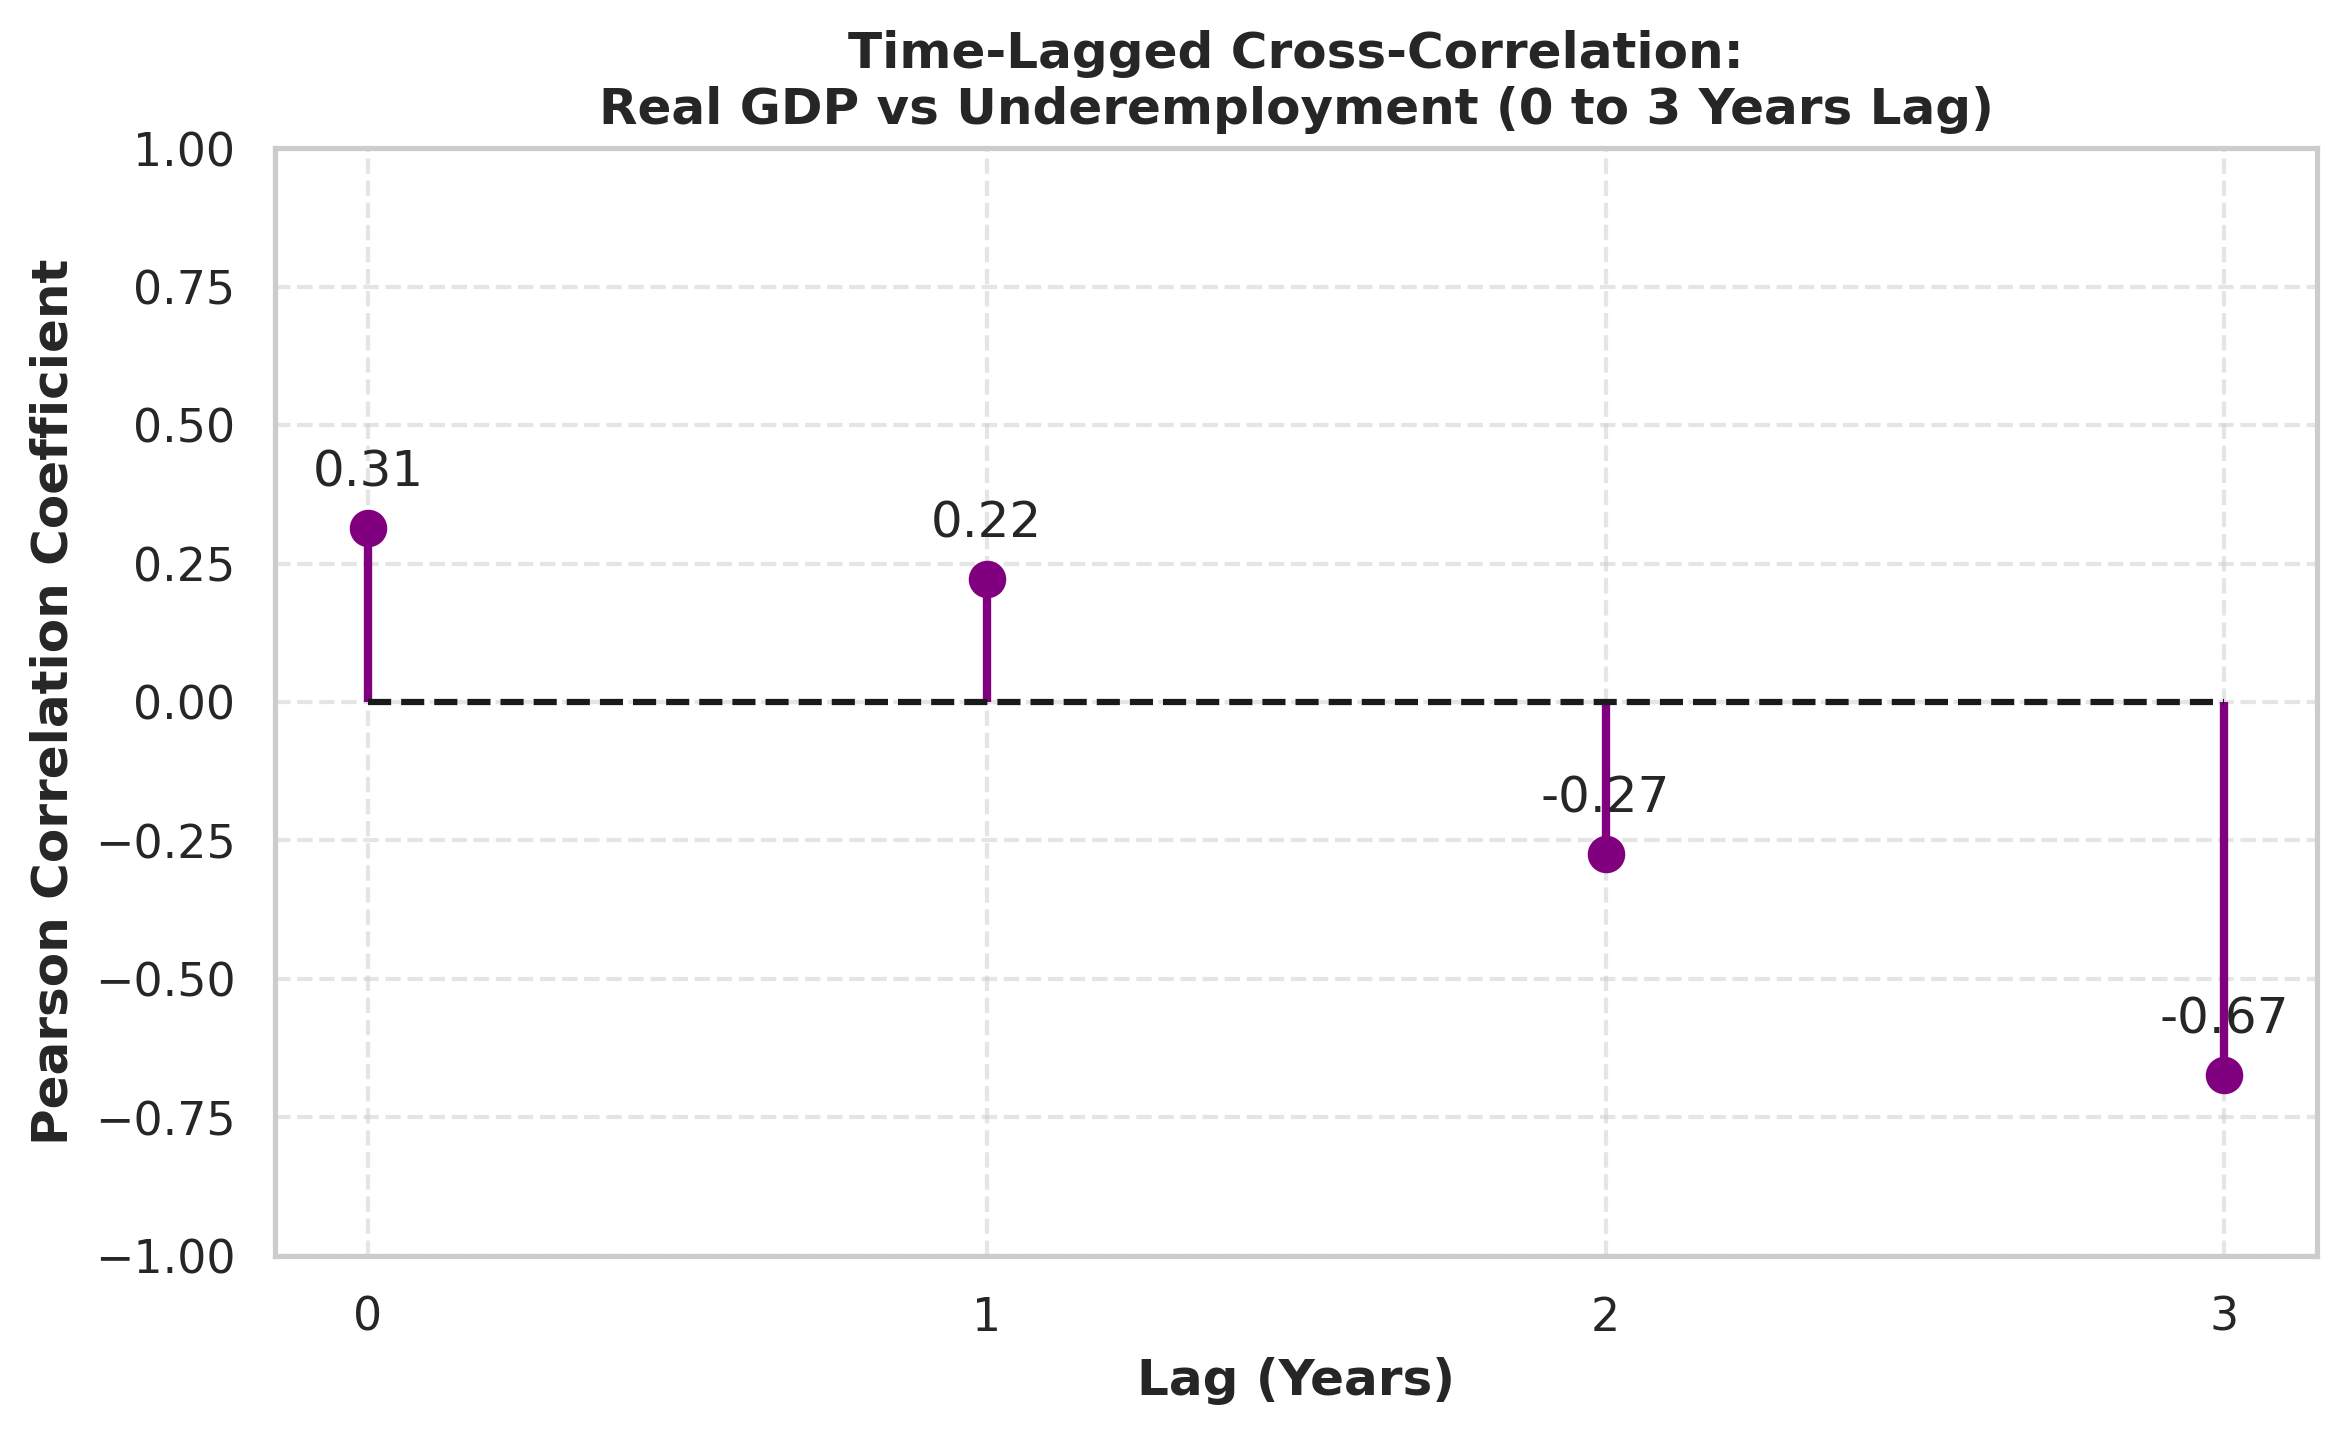
\includegraphics[width=\linewidth, height=3.2cm, keepaspectratio]{Lagged_Correlation_TLCC.png}
  \caption{TLCC matrix. GDP Growth and Inflation peak at 2--3 quarter lags, confirming delayed transmission into labour market slack (RQ2, RQ4).}
  \label{fig:tlcc}
\end{figure}

\subsection{SHAP Feature Association (RQ2)}

The XGBoost model achieves $R^2{>}0.90$. Exchange Rate is excluded consistent with the VIF multicollinearity finding. Figure~\ref{fig:shap} presents SHAP results: \textbf{(1) GDP Contraction} carries the highest mean absolute SHAP value, acting as the primary catalyst---consistent with OLS signs and validating underemployment as a crisis shock absorber. \textbf{(2) Inflation} shows high SHAP density in crisis-year observations, capturing the purchasing-power collapse. \textbf{(3) Youth LFPR and Informal Employment} reflect the qualification-mismatch channel: declining youth LFPR maps to discouraged-worker effects. \textbf{(4)} All top SHAP directions agree with OLS coefficient signs, providing cross-method validation.

\begin{figure}[h]
  \centering
  
\includegraphics[width=\linewidth, height=3.2cm, keepaspectratio]{shap_summary_plots.png}
  \caption{SHAP beeswarm (left) and mean absolute importance (right). GDP Growth and Inflation dominate both panels (RQ2). Exchange Rate excluded due to VIF\,=\,12.28.}
  \label{fig:shap}
\end{figure}

%% ===================================================
\section{Conclusion}
%% ===================================================

Quarterly LFS micro-data reveals crisis underemployment peaks of 32.6\%---nine times the concurrent 3.8\% unemployment rate. Structural break tests (Zivot-Andrews and Bai-Perron PELT) confirm 2021--2022 as a statistically significant rupture in the underemployment--GDP--inflation system, with macro breaks leading the labour market break by one year. VIF analysis identifies Exchange Rate as collinear with Inflation (VIF\,=\,12.28) and excludes it from long-run models. STL decomposition confirms persistent post-crisis trend elevation. SHAP establishes GDP contraction and hyperinflation as dominant drivers, with Youth LFPR and informal employment capturing the qualification-mismatch channel. These findings confirm aggregate unemployment is an inadequate crisis barometer for Sri Lanka.

\textbf{Limitations.} The annual dataset ($n{=}10$) rendered Johansen and full ARDL infeasible; results are directional pending quarterly expansion. Remittances and quarterly agricultural data are absent. The 2024 GDP rate is extrapolated; the 2022 LFS artefact complicates annual inference. STL seasonal estimates at annual frequency are indicative only and should be re-estimated on quarterly data.

\textbf{Future work} will: finalise ARDL on the full quarterly dataset for RQ4 long-run coefficients; generate 2022~Q3 SHAP waterfall and force plots; complete sensitivity analysis across both underemployment definitions; and incorporate remittances and agricultural indices.

\bibliographystyle{ACM-Reference-Format}
\bibliography{references}

\end{document}
